% Compile with: latexmk -pdf dixon.tex
\documentclass[aspectratio=169,11pt,professionalfonts]{beamer}
\usepackage[T1]{fontenc}
\usepackage{lmodern}
\usepackage{amsmath,amssymb,booktabs,array,tikz}
\newcolumntype{L}[1]{>{\raggedright\arraybackslash}p{#1}}
\usetikzlibrary{arrows.meta,positioning,calc}
\definecolor{Ink}{HTML}{142E46}
\definecolor{Teal}{HTML}{087E8B}
\definecolor{Muted}{HTML}{60717F}
\definecolor{Pale}{HTML}{EAF3F5}
\definecolor{Rule}{HTML}{D8E1E7}
\setbeamercolor{normal text}{fg=Ink,bg=white}
\setbeamercolor{structure}{fg=Teal}
\setbeamercolor{frametitle}{fg=Ink,bg=white}
\setbeamertemplate{navigation symbols}{}
\setbeamersize{text margin left=9mm,text margin right=9mm}
\setbeamerfont{frametitle}{size=\Large,series=\bfseries}
\setbeamertemplate{frametitle}{\vspace{3mm}\insertframetitle\par\vspace{1.5mm}{\color{Rule}\hrule}\vspace{1mm}}
\setbeamertemplate{footline}{\hspace{9mm}\color{Muted}\tiny Dixon Resultants for Polynomial System Solving\hfill\insertframenumber\,/\,\inserttotalframenumber\hspace{9mm}\vspace{3mm}}
\setbeameroption{hide notes}
\newcommand{\src}[1]{\vfill{\color{Muted}\fontsize{7}{8.5}\selectfont #1\par}}
\newcommand{\lead}[1]{{\color{Teal}\large #1}\par\vspace{3mm}}
\newcommand{\gap}{\par\vspace{3mm}}
\newcommand{\F}{\mathcal F}
\newcommand{\M}{\mathcal M}
\newcommand{\xx}{\mathbf x}
\newcommand{\avec}{\mathbf a}
\tikzset{box/.style={draw=Rule,fill=Pale,rounded corners=1mm,minimum height=10mm,align=center,font=\small,text=Ink},flow/.style={-{Stealth[length=2mm]},line width=.8pt,draw=Teal},lab/.style={font=\small,text=Muted,align=center}}
\title{Efficient Polynomial System Solving via Dixon Resultants}
\author{Haohai Suo and Jiamin Cui}
\hypersetup{pdftitle={Efficient Polynomial System Solving via Dixon Resultants},pdfauthor={Haohai Suo; Jiamin Cui}}
\begin{document}

% 01
\begin{frame}[plain]
\vspace{10mm}{\LARGE\bfseries Efficient Polynomial System Solving\par via Dixon Resultants\par}
\vspace{4mm}{\large Applications to AO Primitives}\gap\vspace{4mm}
Haohai Suo\qquad Jiamin Cui\par
{\small\color{Muted}Shandong University}\vfill
\note{Plan for 30--40 minutes for the main 30 slides; the four backup slides are for discussion. This talk is based on the uploaded paper. We focus on what Dixon elimination computes, why it is valid, and how the paper improves its analysis and implementation.}
\end{frame}

% 03
\begin{frame}{AO cryptanalysis leads to polynomial systems}
\lead{Arithmetic-friendly rounds admit compact algebraic descriptions.}
\begin{center}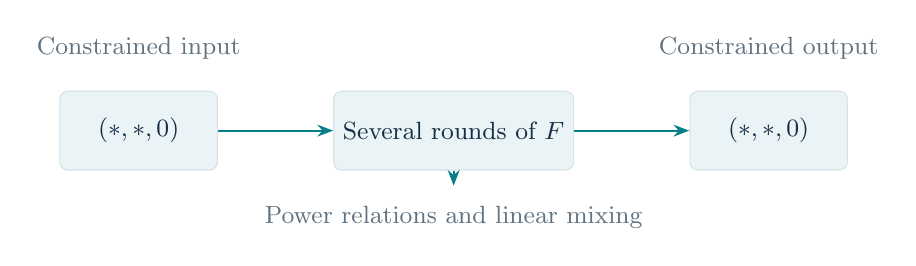
\begin{tikzpicture}
\node[lab] at (0,1.05) {Constrained input};
\node[box,minimum width=2cm] (a) at (0,0) {$(*,*,0)$};
\node[box,minimum width=2.8cm] (b) at (4,0) {Several rounds of $F$};
\node[box,minimum width=2cm] (c) at (8,0) {$(*,*,0)$};
\node[lab] at (8,1.05) {Constrained output};
\draw[flow] (a)--(b);\draw[flow] (b)--(c);
\node[lab] at (4,-1.1) {Power relations and linear mixing};
\draw[flow] (b.south)--(4,-.7);
\end{tikzpicture}\end{center}
\textbf{CICO:} find a state satisfying both endpoint constraints.\gap
Introduce internal variables and solve the induced polynomial equations.
\src{Paper, Section 2. CICO-1 schematic; stars denote free coordinates. AO means arithmetization-oriented.}
\note{Fixing some input and output coordinates produces a constrained-input constrained-output problem. Power maps and mixing layers give polynomial relations in the input and internal states. The diagram suppresses details of any particular permutation.}
\end{frame}

% 04
\begin{frame}{Eliminated variables and retained parameters}
\[\F=\{f_1,\ldots,f_n\}\subseteq\mathbb K[\avec][\xx],\qquad\xx=(x_1,\ldots,x_{n-1}).\]
\begin{columns}[T,onlytextwidth]\column{.46\textwidth}
\textbf{Eliminate $n-1$ variables}\gap
Combine the equations so that $\xx$ no longer appears.
\column{.47\textwidth}
\textbf{Retain $\avec=(a_1,\ldots,a_k)$}\gap
Produce a necessary relation $R(\avec)=0$.
\end{columns}\vspace{6mm}
\textcolor{Teal}{When $k=1$, the output is a univariate polynomial.}\gap
Its roots are candidates; recovery and verification finish the solving task.
\src{Paper, Sections 2 and 5. A valid nonzero determinantal projection requires the stated applicability conditions.}
\note{Here n means the number of equations, and n minus one is the number of eliminated variables. With one retained parameter the original system has equally many variables and equations. More retained parameters are useful for intermediate elimination.}
\end{frame}

% 05
\begin{frame}{Three algebraic routes}
\renewcommand{\arraystretch}{1.8}
\begin{tabular}{@{}L{2.7cm}L{5.5cm}L{4.4cm}@{}}
\toprule\textbf{Method}&\textbf{Basic operation}&\textbf{Typical role}\\\midrule
Gr\"obner bases&Transform the ideal into a useful basis&General system solving\\
Sylvester resultant&Two polynomials, one eliminated variable&Pairwise elimination\\
\textcolor{Teal}{Dixon resultant}&\textcolor{Teal}{Several polynomials and eliminated variables}&\textcolor{Teal}{Simultaneous elimination}\\\bottomrule
\end{tabular}\par\vspace{5mm}
There is no universal winner. Structure, variable count, and degree matter.
\src{Paper, Sections 1--3. GB solving may include an order change; this table does not restrict GB methods to one workflow.}
\note{Gröbner bases also support elimination. Dixon offers a different construction, not an exclusive capability. Its cost profile and treatment of retained variables as parameters can be attractive in certain regimes.}
\end{frame}

% 06
\begin{frame}{The Dixon pipeline}
\begin{center}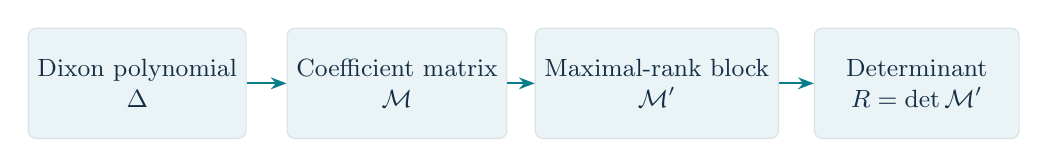
\begin{tikzpicture}
\node[box,minimum width=2.6cm,minimum height=14mm] (a) at (0,0) {Dixon polynomial\\$\Delta$};
\node[box,minimum width=2.6cm,minimum height=14mm] (b) at (3.3,0) {Coefficient matrix\\$\M$};
\node[box,minimum width=2.6cm,minimum height=14mm] (c) at (6.6,0) {Maximal-rank block\\$\M'$};
\node[box,minimum width=2.6cm,minimum height=14mm] (d) at (9.9,0) {Determinant\\$R=\det\M'$};
\draw[flow] (a)--(b);\draw[flow] (b)--(c);\draw[flow] (c)--(d);
\end{tikzpicture}\end{center}\vspace{5mm}
\[\Delta(\xx,\bar\xx)=X\M\bar X^T.\]
\begin{center}$X$ and $\bar X$ list monomials in two sets of variables.\end{center}\vspace{3mm}
\textbf{Main cost drivers:} matrix dimension, entry degrees, and structure.
\src{Paper, Section 2.2. The maximal-rank-block route needs a valid projection condition for singular matrices.}
\note{We will unpack these steps on a system with a square, generically nonsingular matrix. After understanding that clean case, we return to rectangular and rank-deficient matrices.}
\end{frame}

% 07
\begin{frame}{Worked example: three equations in three variables}
\begin{columns}[c,onlytextwidth]\column{.49\textwidth}
\[\left\{\begin{aligned}f_1&=x+y-z=0,\\f_2&=x-y-1=0,\\f_3&=x^2+y^2-5=0.\end{aligned}\right.\]
\column{.45\textwidth}
\textbf{Eliminate:} $x,y$.\gap
\textbf{Retain:} $z$.\gap
\textbf{Goal:} construct a polynomial $R(z)$ that every solution must satisfy.
\end{columns}\vspace{5mm}
\lead{Small enough to calculate by hand, using the actual Dixon construction.}
\src{Teaching example over $\mathbb Q$. The same calculation over $\mathbb F_{17}$ is given in the backup slides.}
\note{Elementary substitution also solves this system, giving an independent check. We use the full Dixon procedure so every matrix entry and every factor is visible. The equation degrees are one, one, and two.}
\end{frame}

% 08
\begin{frame}{Step 1a: build the cancellation matrix}
Introduce auxiliary variables $u,v$. Replace $x$, then $y$, one at a time.
\vspace{3mm}
\[C=\begin{bmatrix}
x+y-z&x-y-1&x^2+y^2-5\\
u+y-z&u-y-1&u^2+y^2-5\\
u+v-z&u-v-1&u^2+v^2-5
\end{bmatrix}.\]
\vspace{3mm}\begin{center}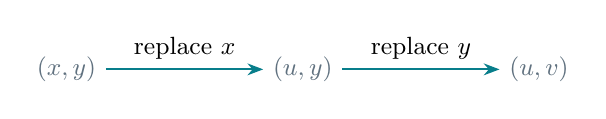
\begin{tikzpicture}
\node[lab] (a) at (0,0) {$(x,y)$};\node[lab] (b) at (3,0) {$(u,y)$};\node[lab] (c) at (6,0) {$(u,v)$};
\draw[flow] (a)--node[above,font=\small] {replace $x$}(b);
\draw[flow] (b)--node[above,font=\small] {replace $y$}(c);
\end{tikzpicture}\end{center}
\src{Dixon construction as defined in the paper, instantiated on the teaching example.}
\note{Each column is one input polynomial. The rows evaluate the same polynomials under progressively more replacements. This pattern forces predictable factors in the determinant.}
\end{frame}

% 09
\begin{frame}{Step 1b: remove the predictable difference factors}
Use consecutive row differences, computed from the original rows:
\[\widehat C_1=C_1,\qquad\widehat C_2=\frac{C_2-C_1}{x-u},\qquad\widehat C_3=\frac{C_3-C_2}{y-v}.\]
\[\widehat C=\begin{bmatrix}x+y-z&x-y-1&x^2+y^2-5\\-1&-1&-(x+u)\\-1&1&-(y+v)\end{bmatrix}.\]
\vspace{1mm}\[\textcolor{Teal}{\Delta=\det\widehat C=\frac{\det C}{(x-u)(y-v)}}.\]
\src{For example, $(u^2-x^2)/(x-u)=-(x+u)$. These are exact polynomial divisions, not numerical divisions at a chosen point.}
\note{The signs follow from later row minus earlier row, divided by original variable minus auxiliary variable. The third row uses original C2. We never divide numerically by zero; the difference quotients are polynomials.}
\end{frame}

% 10
\begin{frame}{Step 2: read off the Dixon matrix}
Expanding the small determinant gives
\[\begin{aligned}\Delta={}&10-(z+1)x+(1-z)y\\&+(2x-z-1)u+(2y-z+1)v.\end{aligned}\]
Choose $X=(1,x,y)$ and $\bar X=(1,u,v)$. Then
\[\Delta=X\,\underbrace{\begin{bmatrix}10&-z-1&1-z\\-z-1&2&0\\1-z&0&2\end{bmatrix}}_{\M(z)}\,\bar X^T.\]
\src{Teaching example. Each entry is the coefficient of one row monomial times one column monomial.}
\note{The coefficient of x times u is two, giving entry (2,2). The coefficient of the constant row monomial times v is one minus z. The resulting matrix has entries in Q[z].}
\end{frame}

% 11
\begin{frame}{Steps 3--4: compute the eliminant and recover solutions}
Our $3\times3$ matrix needs no submatrix extraction. Its determinant is
\[\begin{aligned}R(z)&=40-2(z+1)^2-2(z-1)^2\\&=36-4z^2=\textcolor{Teal}{-4(z^2-9)}.\end{aligned}\]
\begin{columns}[T,onlytextwidth]\column{.46\textwidth}
\textbf{Find candidate roots}\gap $z=3$ or $z=-3$.
\column{.48\textwidth}
\textbf{Recover and verify}\gap $x=(z+1)/2,\quad y=(z-1)/2$.\gap
$(x,y,z)=(2,1,3),\;(-1,-2,-3)$.
\end{columns}
\src{The nonzero factor $-4$ does not affect roots over $\mathbb Q$. Both triples satisfy all three original equations.}
\note{The matrix is nonsingular over Q(z) although singular at the relevant parameter values. This closes the calculation. Back-substitution uses the first two equations and then checks the third.}
\end{frame}

% 12
\begin{frame}{Why is division by $(x-u)(y-v)$ exact?}
\begin{columns}[T,onlytextwidth]\column{.46\textwidth}
\textbf{Set $x=u$}\gap The first two rows of $C$ coincide.\gap Therefore $x-u$ divides $\det C$.
\column{.47\textwidth}
\textbf{Set $y=v$}\gap The last two rows of $C$ coincide.\gap Therefore $y-v$ divides $\det C$.
\end{columns}\vspace{6mm}
These linear factors are relatively prime in the polynomial ring. Thus
\[\det C=(x-u)(y-v)\Delta,\qquad\textcolor{Teal}{\Delta\in\mathbb Q[x,y,u,v,z]}.\]
\src{The general construction removes one predictable difference factor per eliminated variable.}
\note{This is a polynomial identity, not an assumption about numerical auxiliary values. The factor theorem applies because replacing x by u makes the determinant identically zero. Since x minus u and y minus v are distinct relatively prime polynomial factors, their product divides the determinant.}
\end{frame}

% 13
\begin{frame}{Why does a common solution force $R(z)=0$?}
Let $(x_0,y_0,z_0)$ satisfy the three original equations.
\begin{enumerate}\setlength{\itemsep}{3mm}
\item The first row of $C(x_0,y_0,u,v,z_0)$ is zero, so $\det C\equiv0$.
\item The polynomial identity gives
\[(x_0-u)(y_0-v)\Delta(x_0,y_0,u,v,z_0)\equiv0.\]
The first two factors are nonzero polynomials in $u,v$; hence $\Delta\equiv0$.
\item Comparing coefficients of $1,u,v$ yields
\[\textcolor{Teal}{(1,x_0,y_0)\M(z_0)=0}.\]
\end{enumerate}
The vector is nonzero. Therefore $\M(z_0)$ is singular and $\det\M(z_0)=0$.
\src{Polynomial cancellation is in the integral domain $\overline{\mathbb Q}[u,v]$. The evaluation vector includes the constant monomial.}
\note{The cancellation is in the polynomial ring of auxiliary variables. Even if u later equals x0 at some numerical point, x0 minus u is not the zero polynomial. Once Delta is the zero polynomial, every auxiliary-monomial coefficient vanishes. This creates the nonzero left-kernel vector.}
\end{frame}

% 14
\begin{frame}{The kernel vector is visible in the example}
For $(x,y,z)=(2,1,3)$,
\[\M(3)=\begin{bmatrix}10&-4&-2\\-4&2&0\\-2&0&2\end{bmatrix},\qquad X(2,1)=(1,2,1).\]
\vspace{3mm}\[\begin{aligned}(1,2,1)\M(3)&=(10-8-2,\;-4+4,\;-2+2)\\&=(0,0,0).\end{aligned}\]
\vspace{4mm}\lead{A solution becomes a linear dependence in the coefficient matrix.}
\src{Teaching example. This is the concrete linear-algebra mechanism behind the eliminant.}
\note{This multiplication is the key intuition. A nonlinear solution supplies values for the row monomials, and those values annihilate the coefficient matrix. The determinant detects the resulting linear dependence.}
\end{frame}

% 15
\begin{frame}{A resultant root is a necessary condition}
\lead{The converse can fail when degrees drop or extra factors appear.}
Consider two polynomials in $x$, retaining $t$:
\[f_1=tx-1,\qquad f_2=tx-2.\]
Their one-variable Dixon construction gives
\[\frac{\det\begin{bmatrix}tx-1&tx-2\\tu-1&tu-2\end{bmatrix}}{x-u}=-t.\]
At $t=0$ the eliminant vanishes, but the equations become $-1=0$ and $-2=0$.
\gap\textcolor{Teal}{Recover candidates and check them in the original system.}
\src{Teaching counterexample over $\mathbb Q$. Degree degeneration shows why determinant vanishing need not certify an affine solution.}
\note{These equations are inconsistent for every t because their difference is one. The determinant nonetheless has the root zero, where the x-dependent leading terms disappear. This illustrates the false converse without relying on a complicated extra-factor example.}
\end{frame}

% 16
\begin{frame}{Rectangular or singular Dixon matrices}
\begin{columns}[T,onlytextwidth]\column{.46\textwidth}
\textbf{What can happen?}\gap The row and column supports have different sizes.\gap
Or the matrix has generic rank $\rho<D$, even before parameter specialization.
\column{.48\textwidth}
\textbf{Practical route}\gap Evaluate at a generic point, identify independent rows and columns, and extract a $\rho\times\rho$ block.
\end{columns}\vspace{5mm}
\textcolor{Teal}{Two separate checks: preserve rank, and preserve projection validity.}\gap
The KSY/RSC condition supplies a sufficient projection criterion. A nonzero minor alone is not enough.
\src{Paper, Section 2.2 and Appendix F. A random specialization can lose rank; the singular-matrix route requires additional conditions.}
\note{The proof for the generically nonsingular example does not justify arbitrary minors of singular matrices. Rank extraction is linear algebra, while validity as an elimination polynomial is an additional algebraic condition. Backup slide 31 gives a small example of the distinction.}
\end{frame}

% 17
\begin{frame}{Matrix size becomes a lattice-point count}
\begin{columns}[c,onlytextwidth]\column{.46\textwidth}
\begin{center}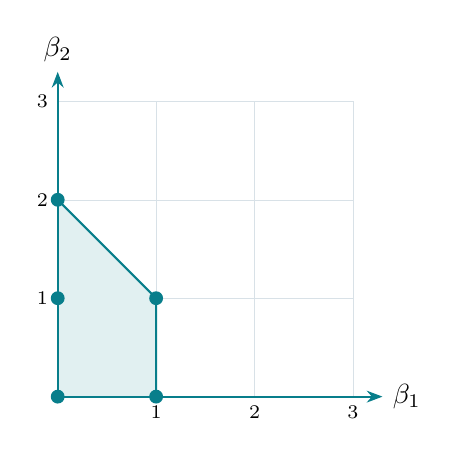
\begin{tikzpicture}[scale=1.25]
\draw[step=1,Rule,very thin] (0,0) grid (3,3);
\fill[Teal!12] (0,0)--(1,0)--(1,1)--(0,2)--cycle;
\draw[flow] (0,0)--(3.3,0) node[right] {$\beta_1$};
\draw[flow] (0,0)--(0,3.3) node[above] {$\beta_2$};
\draw[Teal,thick] (0,2)--(1,1)--(1,0);
\foreach \x/\y in {0/0,0/1,0/2,1/0,1/1}{\fill[Teal] (\x,\y) circle (2pt);}
\foreach \x in {1,2,3}{\node[below,font=\scriptsize] at (\x,0) {\x};}
\foreach \y in {1,2,3}{\node[left,font=\scriptsize] at (0,\y) {\y};}
\end{tikzpicture}\end{center}
\column{.51\textwidth}
\textbf{Three quadratic equations}\gap Monomial exponents obey
\[\beta_1\le1,\qquad\beta_1+\beta_2\le2.\]
{\color{Teal}\Large Five feasible lattice points}\gap Hence $D\le5$.\gap
In higher dimensions, these constraints correspond to bounded lattice paths.
\end{columns}
\src{Paper, Section 3.1. Reverse-ordered exponents are shown. This quadratic illustration is separate from the mixed-degree worked example.}
\note{Every monomial has an exponent vector, which is a lattice point. The construction restricts sums of exponents. Reversing their order gives prefix constraints. Our worked example had degrees one, one, two and a three-by-three matrix; this separate quadratic example illustrates the generic bound five.}
\end{frame}

% 18
\begin{frame}{A sharper bound on the Dixon matrix dimension}
\begin{columns}[c,onlytextwidth]\column{.49\textwidth}
For $n$ equations of degree at most $d$ in the eliminated variables,
\[D\le C_n^{(d)}=\frac{1}{n(d-1)+1}\binom{nd}{n}.\]
\textbf{Fuss--Catalan numbers} count the allowed supports.\gap
Unequal degrees lead to a Hessenberg determinant formula.
\column{.47\textwidth}
\textbf{Example: $n=5$, $d=3$}\gap
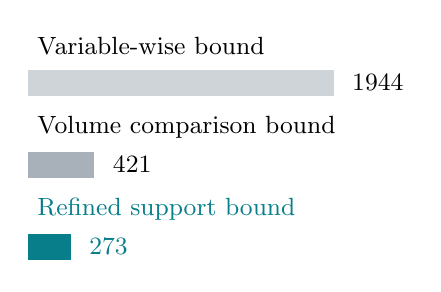
\begin{tikzpicture}[x=.002cm,y=1cm]
\node[anchor=west,font=\small] at (0,.64) {Variable-wise bound};
\fill[Muted!30] (0,0) rectangle (1944,.33);
\node[anchor=west,font=\small] at (2000,.17) {1944};
\node[anchor=west,font=\small] at (0,-.4) {Volume comparison bound};
\fill[Muted!55] (0,-1.04) rectangle (421,-.71);
\node[anchor=west,font=\small] at (480,-.87) {421};
\node[anchor=west,font=\small,text=Teal] at (0,-1.44) {Refined support bound};
\fill[Teal] (0,-2.08) rectangle (273,-1.75);
\node[anchor=west,font=\small,text=Teal] at (330,-1.91) {273};
\end{tikzpicture}
\end{columns}
\src{Paper, Section 3.1 and Appendix C. Generic attainment needs the characteristic hypothesis. Support dimension is not rank; these are bounds, not measured speedups.}
\note{The new support bound is attained generically under a characteristic hypothesis, but this is not a statement about full rank. The bar lengths compare mathematical bounds. They do not show a measured sevenfold matrix reduction or speedup.}
\end{frame}

% 18a
\begin{frame}[t]{Proof framework for the matrix-size bound}
\begin{center}
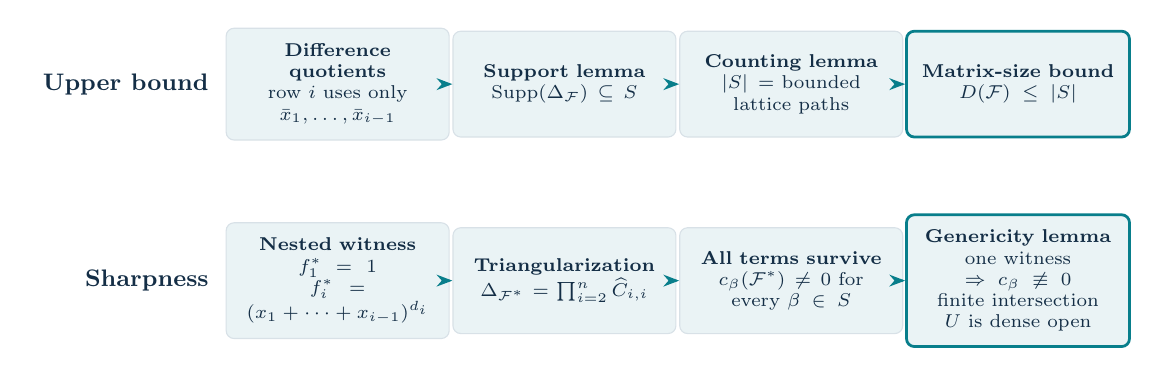
\begin{tikzpicture}[
  scale=.96,transform shape,
  pbox/.style={box,text width=2.55cm,minimum height=14mm,font=\scriptsize},
  every node/.style={inner sep=2mm}
]
\node[anchor=east,font=\small\bfseries,text=Ink] at (-.25,1.35) {Upper bound};
\node[pbox] (structure) at (1.25,1.35)
  {\textbf{Difference quotients}\\row $i$ uses only $\bar x_1,\ldots,\bar x_{i-1}$};
\node[pbox] (support) at (4.25,1.35)
  {\textbf{Support lemma}\\$\operatorname{Supp}(\Delta_{\F})\subseteq S$};
\node[pbox] (paths) at (7.25,1.35)
  {\textbf{Counting lemma}\\$|S|=$ bounded lattice paths};
\node[pbox,draw=Teal,line width=1pt] (bound) at (10.25,1.35)
  {\textbf{Matrix-size bound}\\$D(\F)\le |S|$};
\draw[flow] (structure)--(support);
\draw[flow] (support)--(paths);
\draw[flow] (paths)--(bound);

\node[anchor=east,font=\small\bfseries,text=Ink] at (-.25,-1.25) {Sharpness};
\node[pbox] (witness) at (1.25,-1.25)
  {\textbf{Nested witness}\\$f_1^*=1$\\$f_i^*=$\\$(x_1+\cdots+x_{i-1})^{d_i}$};
\node[pbox] (triangle) at (4.25,-1.25)
  {\textbf{Triangularization}\\$\Delta_{\F^*}=\prod_{i=2}^n\widehat C_{i,i}$};
\node[pbox] (nonzero) at (7.25,-1.25)
  {\textbf{All terms survive}\\$c_\beta(\F^*)\ne0$ for every $\beta\in S$};
\node[pbox,draw=Teal,line width=1pt] (generic) at (10.25,-1.25)
  {\textbf{Genericity lemma}\\one witness $\Rightarrow c_\beta\not\equiv0$\\finite intersection $U$ is dense open};
\draw[flow] (witness)--(triangle);
\draw[flow] (triangle)--(nonzero);
\draw[flow] (nonzero)--(generic);
\end{tikzpicture}
\end{center}
\vspace{1mm}
\begin{center}\small
$|S|=C_n^{(d)}$ in equal degree; unequal degrees give the Hessenberg formula.\par
{\color{Muted}\scriptsize Characteristic $0$ or sufficiently large; support attainment does not assert full rank.}
\end{center}
\src{Paper, Section 3.1 and the proof of the support-bound lemma. Attainment concerns matrix support size, not full rank.}
\note{First prove containment for every determinant term, then count the containing support by lattice paths. For sharpness, the nested witness makes the transformed cancellation matrix upper triangular, and evaluating the original variables at one exposes every allowed dual monomial. A specialization cannot create a dual monomial absent before specialization. More formally, every displayed coefficient is a polynomial in the generic input coefficients; being nonzero at the witness makes its nonvanishing locus open and nonempty. Intersect the finitely many loci, and also their variable-reversed copies, to obtain generic attainment for both row and column supports.}
\end{frame}

% 19
\begin{frame}{Complexity: size and degree both matter}
For one retained parameter, the final polynomial matrix can be handled by HNF:
\[\textcolor{Teal}{T_{\mathrm{det}}=\widetilde O(\rho^\omega E)},\qquad\rho\le D,\quad E\le nd.\]
\begin{columns}[T,onlytextwidth]\column{.46\textwidth}
\textbf{Smaller matrix}\gap Reducing $\rho$ or its bound has a strong effect through $\rho^\omega$.
\column{.48\textwidth}
\textbf{Lower entry degree}\gap Low-degree rows and columns can also reduce determinant work.
\end{columns}\vspace{4mm}
The full symbolic cost includes construction and rank extraction:
\[T_{\mathrm{symbolic}}=\widetilde O\!\left(\max\{T_{\mathrm{construct}},T_{\mathrm{extract}},T_{\mathrm{det}}\}\right).\]
\src{Paper, Sections 2.3 and 3.2. Here $E\ge1$ bounds entry degree and input total degrees are at most $d$. Recovery is separate; construction cannot always be discarded.}
\note{HNF means Hermite normal form. The costs count base-field arithmetic. The paper compares several determinant models because no method is uniformly best. We retain all symbolic stages, especially since the idealized exponent omega equals two does not generally justify ignoring construction.}
\end{frame}

% 20
\begin{frame}{Choosing a submatrix with lower degree}
\lead{Favor low-degree rows and columns while preserving rank.}
\[\deg\det A\le\min\!\left\{\sum\operatorname{rdeg}(A),\;\sum\operatorname{cdeg}(A)\right\}.\]
\renewcommand{\arraystretch}{1.5}
\begin{tabular}{@{}L{6.9cm}rr@{}}
\toprule\textbf{Observed degree test}&\textbf{Random}&\textbf{Degree-aware}\\\midrule
Determinant degree exceeds the B\'ezout bound&963/1000&\textcolor{Teal}{\textbf{1/1000}}\\\bottomrule
\end{tabular}\par\vspace{4mm}
A useful heuristic, with no guarantee of eliminating every extraneous factor.
\src{Paper, Section 4.1 and Appendix G. Five configurations, 200 trials each, over $\mathbb F_{65537}$. Passing the test does not certify a factor-free eliminant.}
\note{The row and column degree sums provide cheap proxies. The experiment measures how often the determinant degree exceeds the Bézout bound. It does not measure all extraneous factors, and we retain the one observed failure.}
\end{frame}

% 21
\begin{frame}{DRSolve: putting the pipeline into practice}
\begin{columns}[T,onlytextwidth]\column{.46\textwidth}
\textbf{Implementation}\gap Open-source C code built on FLINT and PML.\gap
Prime fields, extension fields, and rational arithmetic.
\column{.48\textwidth}
\textbf{Algorithm choices}\gap Several matrix-construction and determinant routines.\gap
Degree-aware submatrix selection and complexity estimation.
\end{columns}\vspace{6mm}
\textcolor{Teal}{Elimination and complete solving are distinct tasks.}\gap
A benchmark should specify which output and which stages are timed.
\src{Paper, Section 4.2. \href{https://github.com/drsolve/drsolve}{github.com/drsolve/drsolve}. Subsequent timings are the paper's reported measurements.}
\note{Efficient polynomial-matrix arithmetic is a major reason the implementation improves over earlier Dixon software. We have not rerun the benchmarks or independently certified identical end-to-end timing boundaries across solvers.}
\end{frame}

% 22
\begin{frame}{Fewer variables and higher degree favor Dixon}
\begin{columns}[c,onlytextwidth]\column{.70\textwidth}
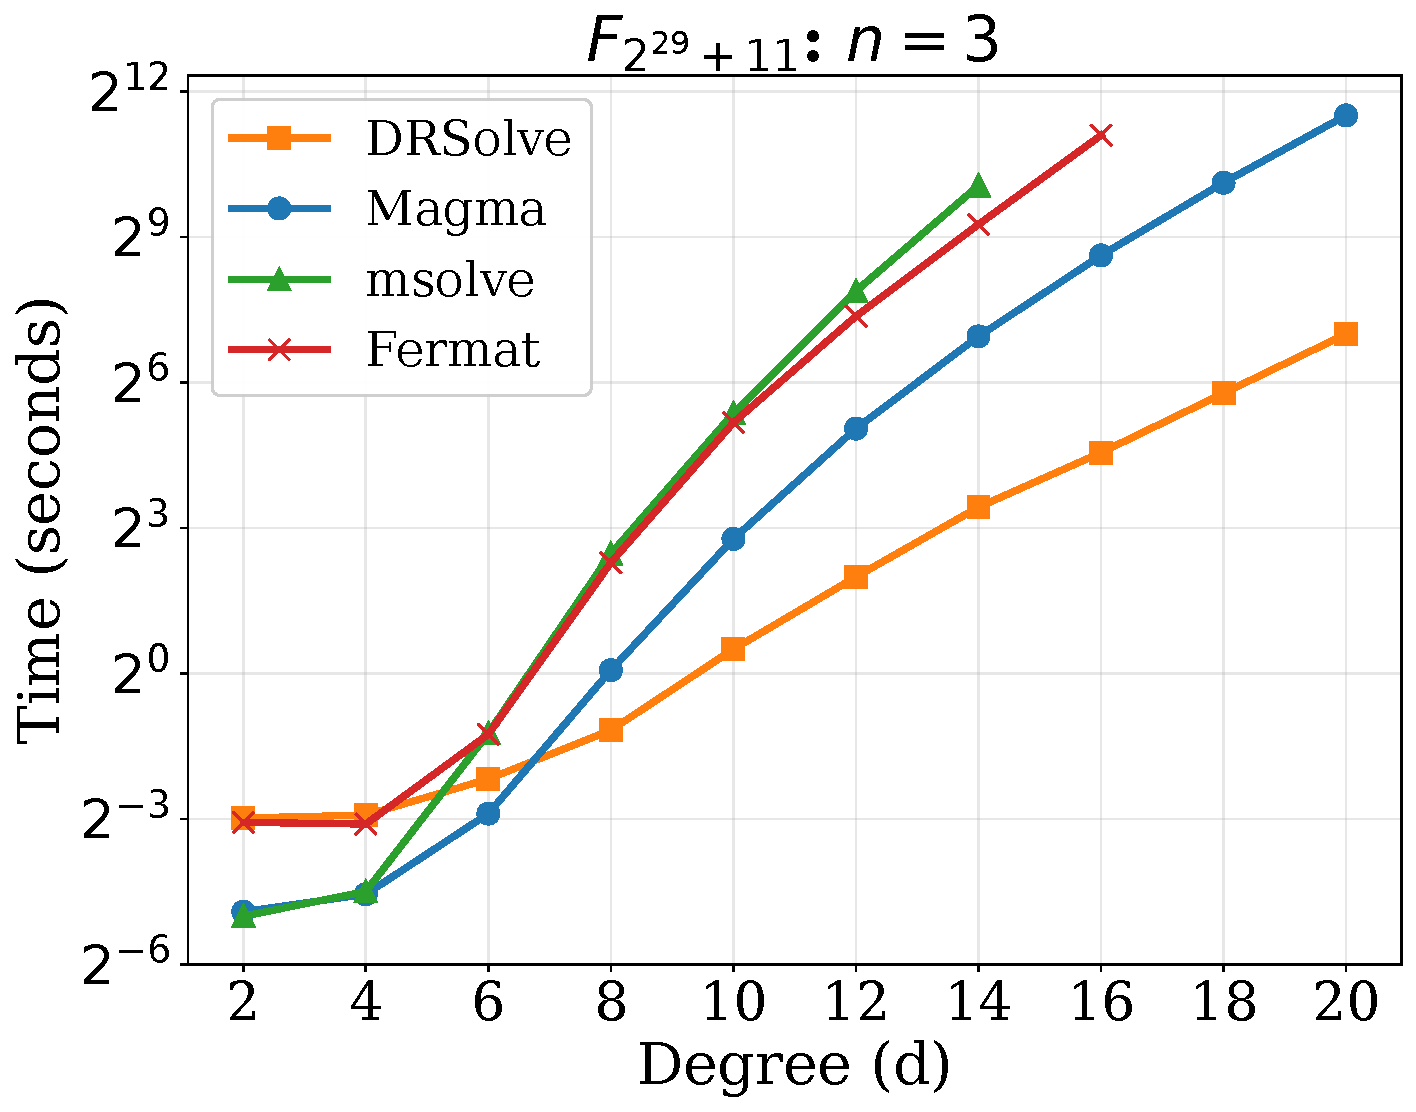
\includegraphics[width=\linewidth,height=5.2cm,keepaspectratio]{assets/benchmark_degree.pdf}
\column{.27\textwidth}
\textbf{Three equations}\gap\textbf{Three variables}\gap
DRSolve is competitive as the degree increases in these tests.
\end{columns}
\src{Paper, Figure 2 ($n=3$ panel). Dense random systems over $\mathbb F_p$, $p=2^{29}+11$. Time in seconds on a log scale. Curves stop at the one-hour timeout.}
\note{Read the curve qualitatively. In this tested family of dense random square systems, DRSolve has the favorable curve at high degree. This is evidence for a regime, not a guarantee about every structured system of a similar degree.}
\end{frame}

% 23
\begin{frame}{More variables and low degree favor GB solvers}
\begin{columns}[c,onlytextwidth]\column{.70\textwidth}
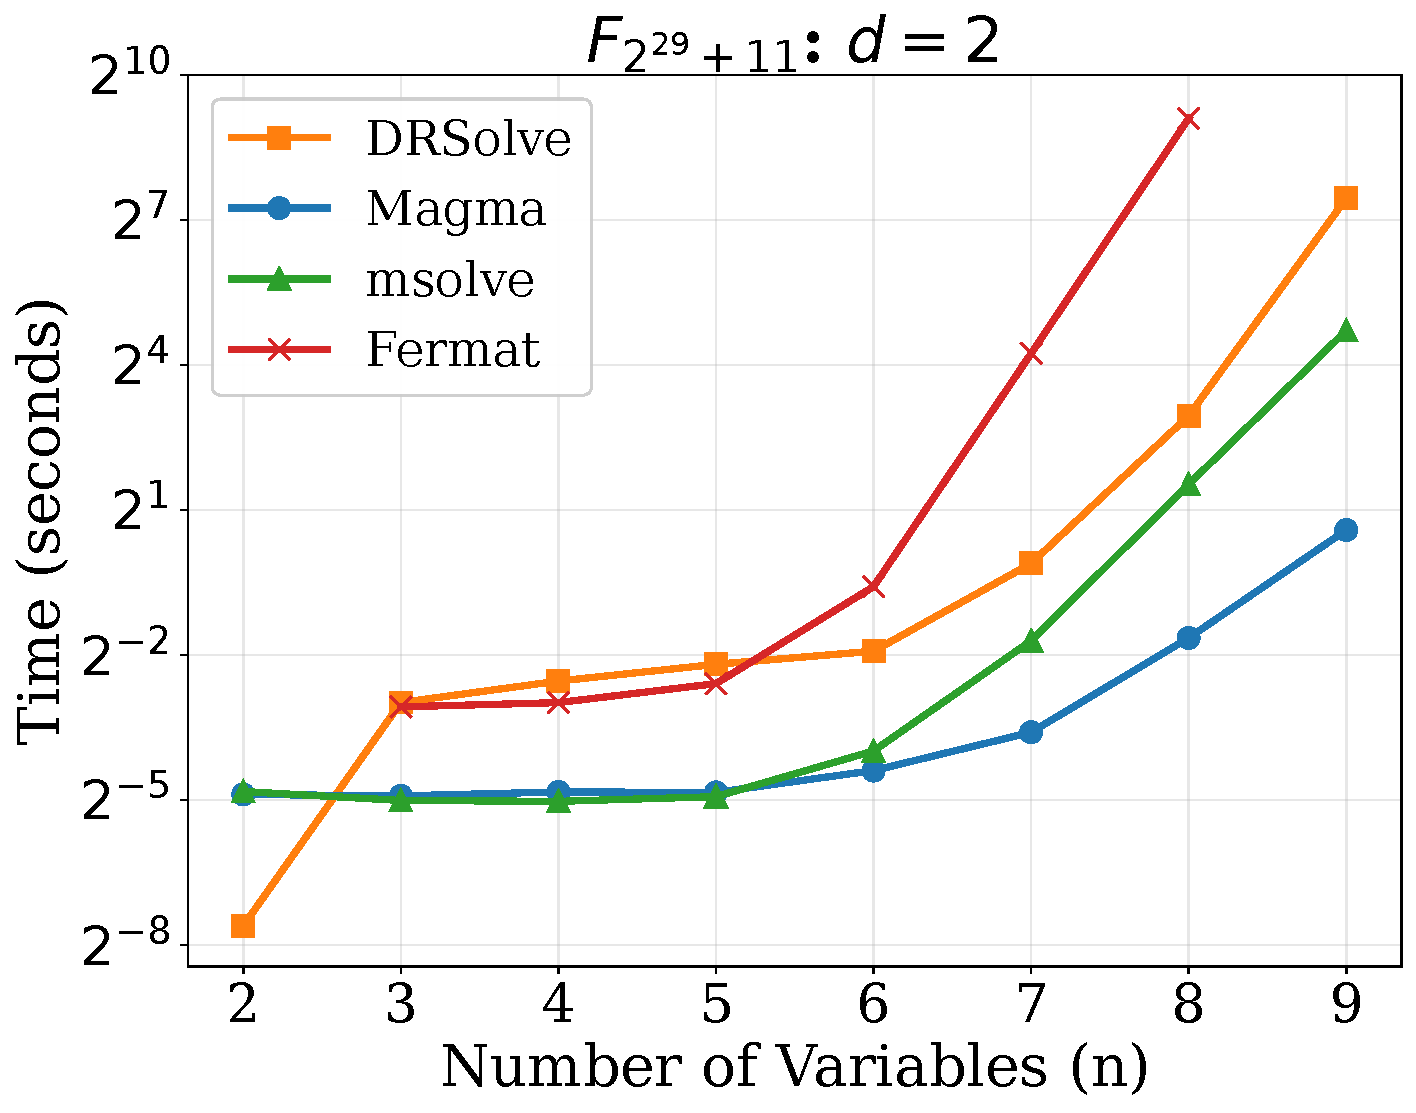
\includegraphics[width=\linewidth,height=5.2cm,keepaspectratio]{assets/benchmark_variables.pdf}
\column{.27\textwidth}
\textbf{Quadratic systems}\gap
As the variable count grows, Magma and msolve remain more competitive.\gap
\textcolor{Teal}{Consider variable count and degree together.}
\end{columns}
\src{Paper, Figure 2 ($d=2$ panel). Equation count equals variable count; same field as the preceding slide.}
\note{This complementary result is important. Practical Gröbner-basis optimizations matter, and the paper does not establish Dixon as the best method for MQ systems. The two plots motivate method selection, not a universal ranking.}
\end{frame}

% 24
\begin{frame}{Three elimination patterns for AO systems}
\renewcommand{\arraystretch}{1.8}
\begin{tabular}{@{}L{2.8cm}L{6.8cm}L{2.6cm}@{}}
\toprule\textbf{Pattern}&\textbf{How it uses structure}&\textbf{Example}\\\midrule
Direct&Eliminate from the complete square system&Poseidon\\
Iterative&Process local relations along a chain&Vision\\
Reduction + elimination&Use triangular relations before merging constraints&XHash12\\\bottomrule
\end{tabular}\par\vspace{5mm}
\lead{The algebraic model determines how elimination should be organized.}
\src{Paper, Section 5. These organizing strategies do not all improve every parameter regime.}
\note{We shift from generic systems to application patterns. The distinguishing structures are a manageable square system, a ladder of local state relations, and a triangular system that permits reduction. No complete round-function description is needed for this level of explanation.}
\end{frame}

% 25
\begin{frame}{Poseidon: direct elimination and structural effects}
\lead{Some small instances favor Dixon; others favor GB.}
\renewcommand{\arraystretch}{1.5}
\begin{tabular}{@{}L{6.8cm}rr@{}}
\toprule\textbf{Configuration $(R_F,R_P,\alpha)$}&\textbf{GB time}&\textbf{Dixon time}\\\midrule
$(3,0,3)$&2.2 s&\textcolor{Teal}{0.3 s}\\
$(4,0,3)$&188189 s&\textcolor{Teal}{1772 s}\\
$(3,1,3)$&\textcolor{Teal}{178 s}&695 s\\
$(2,2,3)$&\textcolor{Teal}{0.4 s}&11.9 s\\\bottomrule
\end{tabular}\par\vspace{3mm}
Partial-round structure can reduce the practical cost of both methods.
\src{Paper, Table 4, selected rows. $t=6,c=1,d=3$, I/O modeling, bypass one round; $p=2^{62}+169$. $R_F,R_P$ denote full and partial rounds.}
\note{Both favorable and unfavorable instances are shown. Partial rounds can influence Dixon supports and ranks, as well as the degree reached by Gröbner-basis computation. Generic upper bounds do not fully predict the resulting practical costs.}
\end{frame}

% 26
\begin{frame}{Vision: meet in a two-variable middle state}
\begin{center}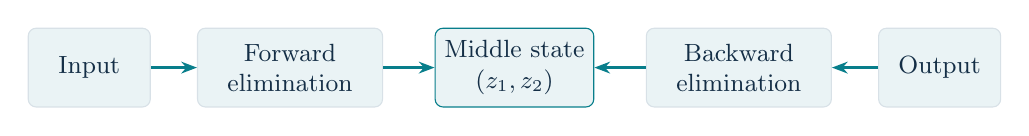
\begin{tikzpicture}
\node[box,minimum width=1.55cm] (a) at (0,0) {Input};
\node[box,minimum width=2.35cm] (b) at (2.55,0) {Forward\\elimination};
\node[box,draw=Teal,minimum width=2cm] (c) at (5.4,0) {Middle state\\$(z_1,z_2)$};
\node[box,minimum width=2.35cm] (d) at (8.25,0) {Backward\\elimination};
\node[box,minimum width=1.55cm] (e) at (10.8,0) {Output};
\draw[flow] (a)--(b);\draw[flow] (b)--(c);\draw[flow] (e)--(d);\draw[flow] (d)--(c);
\end{tikzpicture}\end{center}\vspace{2mm}
\[A(z_1,z_2)=0,\quad B(z_1,z_2)=0\quad\xrightarrow{\ \operatorname{Res}_{z_1}\ }\quad R(z_2)=0.\]
\vspace{3mm}Each chain contributes one relation in the shared middle state.\gap
The final merge dominates the paper's listed stage estimates, subject to its degree assumptions.
\src{Paper, Section 5.2 and Appendix K, $s=2$. The merge eliminates one of two middle variables. Actual determinantal output-degree bounds are conditional.}
\note{The two-variable restriction is essential. Two middle-state relations permit one final one-variable resultant. This does not claim that two equations can eliminate an arbitrarily large middle block. Output-degree assumptions remain part of the estimate.}
\end{frame}

% 27
\begin{frame}{XHash12: reduce powers before eliminating}
\begin{columns}[c,onlytextwidth]\column{.46\textwidth}
\[\begin{aligned}z_1^\alpha&=f_1(\xx),\\z_2^\alpha&=f_2(\xx,z_1),\\&\ \vdots\end{aligned}\]
Triangular relations replace high powers by reduced expressions.
\column{.49\textwidth}
\textbf{The hybrid route}\gap
1. Reduce the output constraints.\gap
2. Eliminate internal variables successively.\gap
3. Merge the input relations with Dixon elimination.
\end{columns}\vspace{4mm}
\textcolor{Teal}{Reduction lowers exponents; it does not itself eliminate all internal variables.}
\src{Paper, Section 5.3 and Appendix L. CICO-1 inherits the optimized pairwise-resultant route of prior work.}
\note{A normal form modulo triangular relations may still contain internal variables. Successive resultant steps are required. With several retained inputs, the final relations must then be merged, and intermediate degree growth may dominate.}
\end{frame}

% 28
\begin{frame}{The hybrid route has its own trade-offs}
\textbf{Paper's symbolic comparison:} strong for CICO-1, a small margin for CICO-2, and worse than direct elimination for CICO-3/4.\par
\vspace{4mm}\textbf{Reported small-instance elimination times}\gap
\renewcommand{\arraystretch}{1.5}
\begin{tabular}{@{}L{5.3cm}rrr@{}}
\toprule\textbf{Instance $(\alpha,\mathrm{width},\mathrm{steps})$}&\textbf{GB}&\textbf{Direct}&\textbf{Hybrid}\\\midrule
CICO-1 $(3,3,5)$&1.5 s&5.12 s&\textcolor{Teal}{0.04 s}\\
CICO-2 $(3,4,3)$&59.7 s&\textcolor{Teal}{4.5 s}&413.2 s\\\bottomrule
\end{tabular}\par\vspace{4mm}
\textcolor{Teal}{A smaller generic cost estimate need not imply a faster small-instance implementation.}
\src{Paper, Figure 5 and Table 6, selected rows. Theoretical and measured comparisons are different kinds of evidence.}
\note{Separate the symbolic upper-bound comparison from measured time. The CICO-2 hybrid example is much slower than direct elimination despite the small generic theoretical margin. Constants, structure and intermediate work matter.}
\end{frame}

% 29
\begin{frame}{What is established, and what remains conditional?}
\begin{columns}[T,onlytextwidth]\column{.47\textwidth}
\textbf{Established structure}\gap Explicit bounds on monomial support.\gap
Generic attainment under the stated characteristic hypothesis.\gap
An elimination implementation and benchmark results.
\column{.47\textwidth}
\textbf{Remaining challenges}\gap Support dimension can greatly exceed rank.\gap
Extraneous-factor control is heuristic.\gap
Structured cryptographic systems need more precise estimates.
\end{columns}
\src{Paper, Sections 3--6. Projection conditions, degree hypotheses, and recovery costs must remain explicit.}
\note{Distinguish the theorem, the heuristic and the experiment. Future opportunities include exploiting rank and support structure, proving stronger factor removal methods, and improving models for specific AO systems.}
\end{frame}

% 30
\begin{frame}{Takeaways}
\vspace{3mm}\begin{enumerate}\setlength{\itemsep}{5mm}
\item A common solution creates a kernel vector in the Dixon matrix.
\item Lattice-path counting sharpens the matrix-size bound.
\item Practical gains depend on variable count, degree, and system structure.
\end{enumerate}\vspace{6mm}
{\color{Teal}\Large Thank you. Questions?}\gap
\href{https://github.com/drsolve/drsolve}{github.com/drsolve/drsolve}
\note{Return to the core mechanism: nonlinear solutions imply linear dependence, so a determinant supplies a necessary relation in the retained variables. The contribution makes this route more tightly estimated and more practical. The next four slides are optional backup material.}
\end{frame}

\appendix
% 31
\begin{frame}{Backup: a nonzero minor alone is not enough}
Consider the abstract polynomial matrix
\[A(t)=\begin{bmatrix}1&t\\0&0\end{bmatrix}.\]
It has a nonzero kernel for every $t$, but a maximal-rank minor is the constant $1$.
\gap\textbf{For a generically singular matrix, singularity itself says nothing new.}\gap
To make maximal minors vanish at solutions, one needs a drop below the generic rank. The Dixon KSY/RSC criterion supplies a sufficient condition in the setting used by the paper.
\src{Illustrative linear-algebra example, not claimed to be a Dixon matrix. See the paper's Section 2.2 for the projection criterion.}
\note{In the nonsingular generic case a nonzero kernel forces determinant zero. A generically singular matrix already has a kernel everywhere, so more is needed. This example shows why arbitrary minor extraction is not a complete elimination correctness argument.}
\end{frame}

% 32
\begin{frame}{Backup: the same example over $\mathbb F_{17}$}
The polynomial identities hold after reduction modulo $17$:
\[R(z)=-4(z^2-9),\qquad z\in\{3,14\}.\]
Since $2^{-1}=9$ in $\mathbb F_{17}$,
\[x=9(z+1),\qquad y=9(z-1)\pmod {17}.\]
\renewcommand{\arraystretch}{1.5}\begin{center}
\begin{tabular}{ccc}\toprule $z$&$x$&$y$\\\midrule 3&2&1\\14&16&15\\\bottomrule\end{tabular}
\end{center}
These are all solutions in $\mathbb F_{17}^3$.
\src{Teaching example. The source package includes exact identity checks and exhaustive verification over $\mathbb F_{17}$.}
\note{No real-number ordering or geometry is needed. The same identities reduce to the finite field. Characteristic seventeen avoids degeneration of the factor four and permits division by two. The verification script exhausts all 4913 triples.}
\end{frame}

% 33
\begin{frame}{Backup: unequal degrees and the worked example}
For sorted positive degree bounds $d_1\le\cdots\le d_n$, set
\[a_i=\sum_{j=1}^{i}(d_{n+1-j}-1).\]
The paper bounds the support dimension by
\[D\le\det_{1\le i,j\le n-1}\left[\binom{a_i+1}{j-i+1}\right].\]
For $(d_1,d_2,d_3)=(1,1,2)$, we have $(a_1,a_2)=(1,1)$:
\[D\le\det\begin{bmatrix}2&1\\1&2\end{bmatrix}=3.\]
\src{Paper, Section 3.1. The worked example's $3\times3$ matrix attains this support-dimension bound. Generic support attainment does not assert full rank in general.}
\note{This connects the hand calculation to the mixed-degree result. The smallest degree does not enter this nested-support formula. The two largest degree bounds, minus one, determine the prefix budgets.}
\end{frame}

% 34
\begin{frame}{Backup: selected references}
\small\begin{itemize}\setlength{\itemsep}{3mm}
\item H. Suo and J. Cui. \emph{Efficient Polynomial System Solving via Dixon Resultants: Applications to AO Primitives}. Uploaded full version.
\item A. L. Dixon (1909). Original multivariate resultant construction.
\item D. Kapur, T. Saxena and L. Yang (1994). Dixon-based resultant algorithms and the singular-matrix setting.
\item G. Labahn, V. Neiger and W. Zhou (2017). Fast univariate polynomial-matrix determinant and Hermite-form algorithms.
\end{itemize}\vspace{3mm}
\href{https://eprint.iacr.org/2026/1969}{eprint.iacr.org/2026/1969}\qquad\href{https://github.com/drsolve/drsolve}{github.com/drsolve/drsolve}
\src{Full bibliographic details and the application-specific literature are in the uploaded paper.}
\note{These are reading pointers. All experimental values are from the uploaded paper. The hand-worked examples are explanatory additions, not claimed as new research contributions.}
\end{frame}
\end{document}
